%%%%%%%%%%%%%%%%%%%%%%%%%%%%%%%%%%%%%%%%%%%%%%%%%%%%%%%%%%%%%%%%%%%%%%
%
% 天文部誌「Super Nova」 使用エンジン:LuaLaTeX
%
% updated 09 Apr, 2021
%
% (c) Yosuke MORIYAMA
% 上記の行を残してつかうこと.2次配布可.ご利用は計画的に.
%
%%%%%%%%%%%%%%%%%%%%%%%%%%%%%%%%%%%%%%%%%%%%%%%%%%%%%%%%%%%%%%%%%%%%%%

\documentclass{classes/supernova}% 天文部誌用のプリアンブル・マクロの読込み
%\usepackage[backend=biber,style=ieee]{biblatex}
%\bibliography{references.bib}
\usepackage{tcolorbox}
\tcbuselibrary{raster,skins,breakable}

\def\vector#1{\mbox{\boldmath $#1$}}
\newcommand{\AmSLaTeX}{%
	$\mathcal A$\lower.4ex\hbox{$\!\mathcal M\!$}$\mathcal S$-\LaTeX}
\newcommand{\PS}{{\scshape Post\-Script}}
\def\BibTeX{{\rmfamily B\kern-.05em{\scshape i\kern-.025em b}\kern-.08em
T\kern-.1667em\lower.7ex\hbox{E}\kern-.125em X}}
\newcommand{\DeLta}{{\mit\Delta}}
\renewcommand{\d}{{\rm d}}
\def\wcaption#1{\caption[]{\parbox[t]{100mm}{#1}}}
\def\rm#1{\mathrm{#1}}
\def\tempC{^\circ \rm{C}}

\makeatletter
\def\@seccntformat#1{\@ifundefined{#1@cntformat}%
	{\csname the#1\endcsname\quad}%      default
	{\csname #1@cntformat\endcsname}%    enable individual control
}
\makeatother
\newcommand{\Azusection}[3]{
	\phantomsection
	\addcontentsline{toc}{section}{#1}
	\begin{tcolorbox}[enhanced,empty,left skip=0pt,left=5pt,
			coltitle=white,title={\textbf{#1}},sharp corners,
			overlay={
					\begin{tcbclipframe}
						\fill[black] (title.south west)--++(#2,0)--++(0,1)--++(-#2,0)--cycle;
					\end{tcbclipframe}}]
		#3
	\end{tcolorbox}
}

\newcommand{\tenexp}[2]{#1\times10^{#2}} % 国分梓用プリアンブル
\usepackage{ascmac}
%%% 女の子と結婚したい.tex  %%%
%%%  幸せになりたい.pdf    %%%

%how to compile and convert to pdf
%platex main.tex
%dvipdfmx main


\newcount\K % int K  
\def\mylove{\K=0 \loop\ifnum\K<100
	女の子が好きだった...。\advance\K by1\repeat}
\newcommand{\piasec}[1]{
	\phantomsection
	\addcontentsline{toc}{section}{#1}
	\section*{#1}
} % 女の子と結婚したい.tex

%%%%%%%%   表紙・ごあいさつ・目次   %%%%%%%%%
\begin{document}
\gtfamily\sffamily % 本文をゴシック体サンセリフ体に統一する
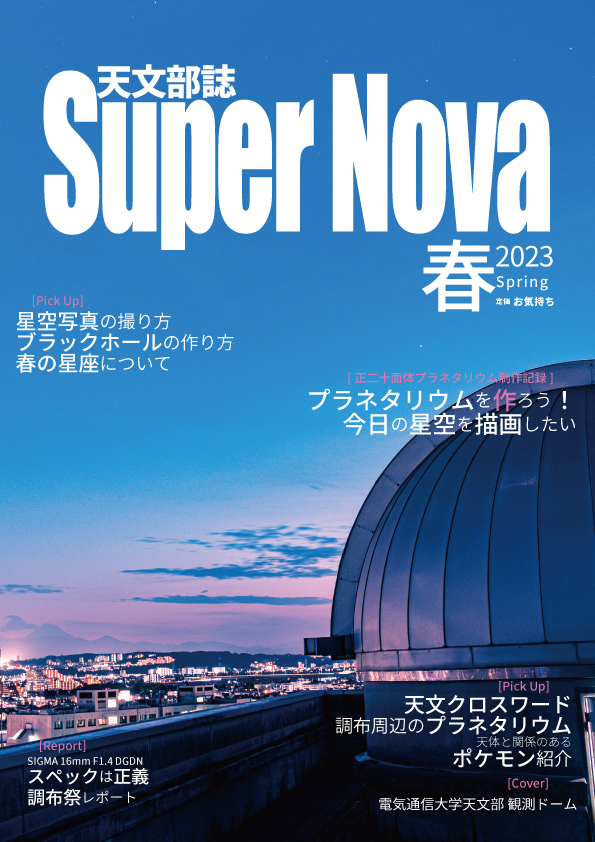
\includepdf[noautoscale=true, fitpaper]{cover/2023spring_supernova_cover.pdf} %表紙
% \maketitle %簡単に済ませる用
\frontmatter
\setcounter{page}{1} %ページカウンタのセット
\subfile{sections/goaisatu} % ご挨拶ページ
\setcounter{tocdepth}{1} % 目次に表示する見出しの深さ指定 0:chapter 1:section 2:subsection 3:subsubsection
\tableofcontents % 目次
\cleartooddpage% 奇数ページまでジャンプ

\mainmatter
%%%%%%%%%   ここから本編   %%%%%%%%
% \subfile{hogehoge} % hogehoge.texを読み込む
\subfile{sections/Mizuyoshi/main} % 調布祭レポート 3p 
\subfile{sections/Ikeda/main} % 春の星座について 5p
\subfile{sections/Azusa/main} % ブラックホールを作ろう! 1p
\subfile{sections/Nakahara/main} % プラネタリウムを作ろう! 3p
\subfile{sections/Tadachi/main} % 今日の星空を描画したい 1p
\subfile{sections/Karasawa/main} % 調布周辺のプラネタリウム 2p
\subfile{sections/Kawaguchi/key} % 天文クロスワード 2p
\subfile{sections/YamaYama/main} % 天文と関係のあるポケモン紹介 2p
\subfile{sections/Maruyama/main} % スペックは正義 6p
\subfile{sections/Yosuke/Orion} % 調布でオリオン大星雲 5p
%%%%%%%%   付録・編集後記   %%%%%%%%
\appendix
% \subfile{appendix} % 付録
\subfile{sections/Yosuke/Photo}
\backmatter % あとがき、編集後記はこの下に
\subfile{sections/kouki} % 編集後記
%\printbibliography[title=参考文献]
%\addcontentsline{toc}{chapter}{参考文献}
\includepdf[noautoscale=true, fitpaper]{cover/2023_spring_atogaki.pdf}
\cleardoublepage
\cleartoevenpage % 奇数ページまでジャンプ
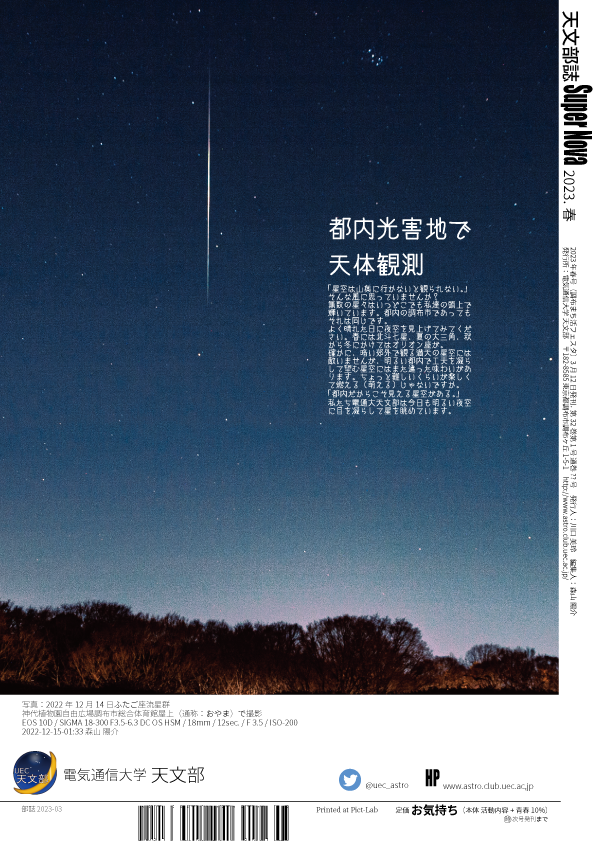
\includepdf[noautoscale=true, fitpaper]{cover/2023spring_supernova_cover_back.pdf} % 裏表紙
\end{document}